
\documentclass[11pt,compress,t,notes=noshow, xcolor=table]{beamer}
% alternatively combining latex files with subfile package https://tex.stackexchange.com/a/155883/26830 (however, page numbering and some other stuff does not work well)

\input{../../style/preamble}
\input{../../latex-math/basic-math}
\input{../../latex-math/basic-ml}

% deactivate beamer navigation
% \setbeamertemplate{navigation symbols}{}
% \usepackage{geometry}
% \geometry{papersize={180mm, 135mm}, top=-1.5mm} % 210mm, 297mm

% set path of iml lecture here, e.g., relative to the current dir
% \usepackage[nospeakermargin]{../../style/lmu-lecture-2}
% \usepackage{pax}
% \setbeamertemplate{frametitle}{\expandafter\uppercase\expandafter\insertframetitle}
%\useoutertheme{metropolis}
% remove section slides
% \AtBeginSection[]
% {
% 	\begin{frame}<beamer>
% 		\frametitle{Applied Machine Learning}
% 		\tableofcontents[currentsection]
% 	\end{frame}
% }
% includepdf slides, pagecommad will set counter for framenumber
\usepackage{pdfpages}
\includepdfset{trim=0mm 0mm 0mm 0mm, pagecommand={\global\setcounter{framenumber}{\value{page}}}}
% trim=0mm 6mm 0mm 0mm, offset=0 15,
% add footer:
\usepackage{framed, color}
\usepackage{xcolor}
\iffalse
\setbeamertemplate{footline}[text line]{%
	\noindent\hspace*{\dimexpr-\oddsidemargin-1in\relax}%
	\colorbox{white}{
		\makebox[\dimexpr\paperwidth-2\fboxsep\relax]{
			\color{black}
			\begin{minipage}[c][2ex][c]{0.5\linewidth}
				\secname
			\end{minipage}
			\hfill\begin{minipage}[c][2ex][c]{0.5\linewidth}
				\flushright
				\insertframenumber{}~/~\inserttotalframenumber~~
			\end{minipage}
	}}%
	\hspace*{-\paperwidth}
}
\fi

\title{Applied Machine Learning}

\begin{document}


\titlemeta{
Machine Learning in R:
}{
mlr 3}{
figure_man/mlr3_logo.png
}{
\item Basics of mlr3: \\Train, Predict, Evaluate
\item Resampling in mlr3
\item Benchmarking in mlr3
}


\includepdf[pages={7-8, 10-18}]{../mlr3slides/mlr3-intro.pdf}

\subsection{Data and Tasks}
\includepdf[pages={24, 26, 30-31}]{../mlr3slides/mlr3-intro.pdf}

\subsection{Dictionaries}
\includepdf[pages={33-36}]{../mlr3slides/mlr3-intro.pdf}

\subsection{Learner}
\includepdf[pages={39-40, 42, 44-50}]{../mlr3slides/mlr3-intro.pdf}

\subsection{Prediction and Evaluation}
\includepdf[pages={51-53, 55-59, 62-65, 67-71}]{../mlr3slides/mlr3-intro.pdf}

% \section{Exercise: Train, predict, evaluate}
% \begin{frame}{Exercise: Train, predict, evaluate}
% File: \textit{day1\_train\_predict\_evaluate.html}
% \end{frame}
\section{Resampling with mlr3}
\includepdf[pages={3, 5, 8-9, 11, 13, 18-23, 27-31}]{../mlr3slides/mlr3-resampling.pdf}
% \section{Exercise: Resampling with mlr3}
% \begin{frame}{Exercise: Resampling with mlr3}
% File: \textit{day1\_resampling.html}
% \end{frame}
\section{Benchmarking with mlr3}
\includepdf[pages={33-36, 40-41, 43}]{../mlr3slides/mlr3-resampling.pdf}

\section{Help and Summary}
\includepdf[pages={45-46, last}]{../mlr3slides/mlr3-resampling.pdf}
% \section{Exercise: Benchmarking with mlr3}
% \begin{frame}{Exercise: Benchmarking with mlr3}
% File: \textit{day1\_benchmarking.html}
% \end{frame}



\endlecture
\end{document}
